\documentclass[conference]{IEEEtran}
\usepackage{amsmath,amssymb,amsfonts}
\usepackage{algorithmic}
\usepackage{algorithm}
\usepackage{array}
\usepackage{graphicx}
\usepackage{textcomp}
\usepackage{xcolor}
\usepackage{booktabs}
\usepackage{listings}
\usepackage{tikz}
\usepackage{pgfplots}
\pgfplotsset{compat=1.18}
\usetikzlibrary{shapes,arrows,positioning,fit,calc}
\usepackage{subcaption}

% Configure listings to prevent column overflow
\lstset{
  breaklines=true,
  breakatwhitespace=true,
  columns=flexible,
  keepspaces=true,
  linewidth=\columnwidth,
  basicstyle=\small\ttfamily,
  postbreak=\mbox{\textcolor{red}{$\hookrightarrow$}\space},
}

\begin{document}

\title{Elastic Dictionary: A Dynamic Hierarchical Data Structure for Semantic Organization}

\author{
    \IEEEauthorblockN{M. Soleymani}
    \IEEEauthorblockA{Department of Computer Science\\
    Advanced AI Research\\
    msoleymani@example.edu}
}

\maketitle

\begin{abstract}
This paper introduces the Elastic Dictionary, an adaptive hierarchical data structure designed to dynamically organize textual information based on semantic similarity. Unlike traditional dictionaries with fixed structures, the Elastic Dictionary evolves as data is added, automatically organizing related concepts into a semantic tree without predefined categories. We leverage sentence embeddings to capture meaning, hierarchical clustering to form categories, and visualization techniques to explore the resulting structure. The implementation addresses compatibility challenges in the clustering algorithms by providing a robust fallback mechanism. We evaluate the structure's performance across multiple test scenarios, demonstrating how it adapts to various domains and restructures to maintain an organized hierarchy. Results show that the Elastic Dictionary successfully identifies and groups semantically related information, facilitating both browsing and semantic search across heterogeneous data.
\end{abstract}

\begin{IEEEkeywords}
semantic search, hierarchical data structures, dynamic clustering, sentence embeddings, adaptive categorization
\end{IEEEkeywords}

\section{Introduction}

Traditional data structures for organizing textual information often require predefined categories or taxonomies, limiting their ability to adapt to new domains or unexpected data patterns. Meanwhile, flat structures like standard dictionaries provide little context for understanding relationships between entries. These limitations become increasingly problematic as the volume and diversity of textual data continue to grow.

The Elastic Dictionary addresses these challenges by providing a dynamic data structure that organizes information based on semantic meaning rather than arbitrary categories. By leveraging recent advances in natural language processing, particularly sentence embeddings, this structure adapts and evolves as new information is added, creating a hierarchical tree that reflects the inherent semantic relationships within the data.

Key contributions of this work include:

\begin{itemize}
    \item A novel dynamic data structure that combines embedding-based similarity with hierarchical organization
    \item Algorithms for optimal placement of new items and periodic restructuring of the tree
    \item Robust implementation techniques that address compatibility issues across different environments
    \item Visualization methods for exploring the evolving semantic structure
    \item Evaluation across multiple domains demonstrating the structure's adaptability
\end{itemize}

This paper is organized as follows: Section II describes the methods and algorithms used to implement the Elastic Dictionary, Section III presents experimental results across various test scenarios, Section IV discusses the implications and challenges, and Section V concludes with a summary and future work.

\section{Methods}

The Elastic Dictionary is built on three foundational concepts: semantic understanding through embeddings, dynamic tree structuring, and adaptive restructuring. This section details the key components and algorithms that implement these concepts.

\subsection{System Architecture}

The core architecture consists of two primary classes: the Node class, which represents individual entries in the dictionary, and the ElasticDictionary class, which manages the overall structure and operations. Figure \ref{fig:architecture} illustrates the high-level system architecture.

\begin{figure}[ht]
\centering
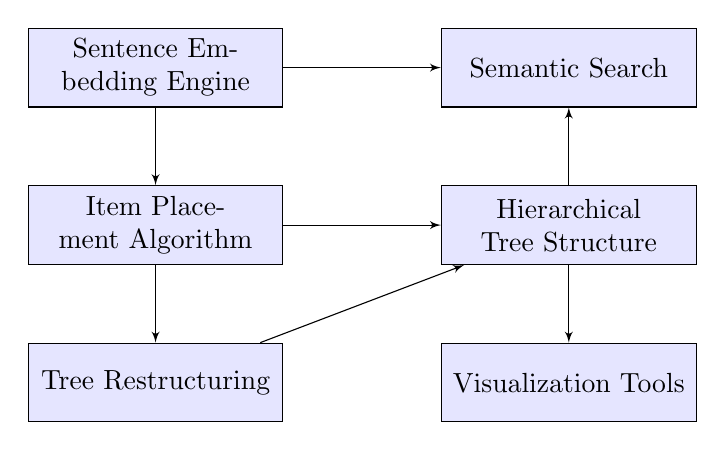
\begin{tikzpicture}[
    node distance = 2cm,
    box/.style = {rectangle, draw, text width=3cm, text centered, minimum height=1cm, fill=blue!10},
    line/.style = {draw, -latex'},
    cloud/.style = {draw, ellipse, fill=red!10, text width=2.5cm, text centered, minimum height=1cm}
]
\node[box] (embedding) {Sentence Embedding Engine};
\node[box, below of=embedding] (placement) {Item Placement Algorithm};
\node[box, below of=placement] (restructuring) {Tree Restructuring};
\node[box, right=2cm of placement] (tree) {Hierarchical Tree Structure};
\node[box, right=2cm of embedding] (search) {Semantic Search};
\node[box, right=2cm of restructuring] (visualization) {Visualization Tools};

\path[line] (embedding) -- (placement);
\path[line] (placement) -- (restructuring);
\path[line] (embedding) -- (search);
\path[line] (placement) -- (tree);
\path[line] (restructuring) -- (tree);
\path[line] (tree) -- (visualization);
\path[line] (tree) -- (search);
\end{tikzpicture}
\caption{Elastic Dictionary system architecture showing the key components and their relationships.}
\label{fig:architecture}
\end{figure}

\subsection{Semantic Embedding}

The foundation of the Elastic Dictionary is the ability to represent textual data as dense vector embeddings that capture semantic meaning. We use the SentenceTransformer library with the "all-MiniLM-L6-v2" model to generate these embeddings. The embedding process is encapsulated in the following method:

\begin{lstlisting}[language=Python]
def _get_embedding(self, text: str) -> np.ndarray:
    """Generate embedding for a text."""
    return self.model.encode(text, show_progress_bar=False)
\end{lstlisting}

\subsection{Item Placement Algorithm}

When a new item is added to the dictionary, it must be placed in an appropriate location in the tree. The placement algorithm recursively traverses the tree to find the most semantically similar node, using cosine similarity as the similarity metric. Algorithm \ref{alg:placement} outlines this process.

\begin{algorithm}
\caption{Item Placement Algorithm}
\label{alg:placement}
\begin{algorithmic}[1]
\REQUIRE New item embedding $e$, Current node $n$ (default: root)
\ENSURE Best node for placement and similarity score
\IF{$n$ has no children}
    \IF{$n$ is root}
        \RETURN $(n, 0.0)$
    \ELSE
        \STATE $sim \gets CosineSimilarity(e, n.embedding)$
        \RETURN $(n, sim)$
    \ENDIF
\ENDIF
\STATE $currSim \gets 0.0$
\IF{$n$ is not root AND $n.embedding$ is not null}
    \STATE $currSim \gets CosineSimilarity(e, n.embedding)$
\ENDIF
\STATE $bestChild \gets null$
\STATE $bestSim \gets 0.0$
\FOR{each child $c$ in $n.children$}
    \IF{$c.embedding$ is not null}
        \STATE $childSim \gets CosineSimilarity(e, c.embedding)$
        \IF{$childSim > bestSim$}
            \STATE $bestSim \gets childSim$
            \STATE $bestChild \gets c$
        \ENDIF
    \ENDIF
\ENDFOR
\IF{$bestSim > minSimilarityThreshold$ AND $bestChild$ is not null}
    \STATE $(childBestNode, childBestSim) \gets$ PLACEMENT($e$, $bestChild$)
    \IF{$childBestSim > currSim$}
        \RETURN $(childBestNode, childBestSim)$
    \ENDIF
\ENDIF
\RETURN $(n, currSim)$
\end{algorithmic}
\end{algorithm}

\subsection{Tree Restructuring}

As the tree grows, it may become unbalanced or contain clusters of semantically similar items that should be grouped together. The restructuring algorithm periodically reorganizes the tree to improve its structure. This involves:

\begin{enumerate}
    \item Collecting all leaf nodes (non-category nodes)
    \item Extracting embeddings for these nodes
    \item Performing hierarchical clustering to identify groups
    \item Creating category nodes for each cluster
    \item Reorganizing the tree to reflect the new structure
\end{enumerate}

A critical component of the restructuring process is the clustering algorithm. We implemented a robust approach that handles compatibility issues with different scikit-learn versions:

\begin{lstlisting}[language=Python]
# Use our simple clustering method instead of scikit-learn's
try:
    # First try using scikit-learn for better performance
    cluster_labels = AgglomerativeClustering(
        n_clusters=max_clusters, 
        linkage='average'
    ).fit_predict(node_embeddings)
except Exception as e:
    print(f"Scikit-learn clustering failed: {e}")
    print("Falling back to simple clustering implementation")
    # Fall back to our simple implementation
    cluster_labels = self._simple_clustering(node_embeddings, max_clusters)
\end{lstlisting}

The fallback clustering algorithm, \texttt{\_simple\_clustering}, implements hierarchical clustering from first principles, avoiding dependencies on specific library implementations. This approach provides robustness across different environments and scikit-learn versions.

\subsection{Custom Clustering Algorithm}

Our custom clustering implementation follows the standard approach to agglomerative clustering, starting with each item in its own cluster and progressively merging the closest clusters until the desired number of clusters is reached. Algorithm \ref{alg:clustering} details this implementation.

\begin{algorithm}
\caption{Simple Hierarchical Clustering}
\label{alg:clustering}
\begin{algorithmic}[1]
\REQUIRE Embeddings matrix $E$, Number of clusters $k$
\ENSURE Cluster labels for each embedding
\STATE $n \gets$ Number of embeddings in $E$
\STATE $S \gets$ Compute similarity matrix using $E$
\STATE $D \gets 1 - S$ \COMMENT{Convert to distance matrix}
\STATE $labels \gets [0, 1, ..., n-1]$ \COMMENT{Initial clusters}
\STATE $activeClusters \gets \{0, 1, ..., n-1\}$
\WHILE{$|activeClusters| > k$}
    \STATE $minDist \gets \infty$
    \STATE $mergeA, mergeB \gets -1, -1$
    \FOR{$i \gets 0$ to $n-1$}
        \IF{$labels[i] \not\in activeClusters$}
            \STATE continue
        \ENDIF
        \FOR{$j \gets i+1$ to $n-1$}
            \IF{$labels[j] \not\in activeClusters$ OR $labels[i] = labels[j]$}
                \STATE continue
            \ENDIF
            \IF{$D[i,j] < minDist$}
                \STATE $minDist \gets D[i,j]$
                \STATE $mergeA \gets labels[i]$
                \STATE $mergeB \gets labels[j]$
            \ENDIF
        \ENDFOR
    \ENDFOR
    \IF{$mergeA \neq -1$ AND $mergeB \neq -1$}
        \STATE Replace all occurrences of $mergeB$ with $mergeA$ in $labels$
        \STATE Remove $mergeB$ from $activeClusters$
    \ENDIF
\ENDWHILE
\STATE Relabel clusters to consecutive integers
\RETURN $labels$
\end{algorithmic}
\end{algorithm}

\subsection{Visualization}

Two visualization methods were implemented to explore the structure of the Elastic Dictionary:

\begin{enumerate}
    \item A static 2D visualization using matplotlib and networkx, which displays the tree structure with labeled nodes.
    \item An interactive 3D visualization using Plotly, which allows for rotation, zooming, and exploration of the tree structure with color-coded nodes (categories in orange, regular items in blue, and the root in green).
\end{enumerate}

These visualizations help users understand how the data is organized and how new items find their place in the hierarchy.

\section{Results}

We evaluated the Elastic Dictionary using three test scenarios: a basic usage example, an advanced example with paragraph processing, and a restructuring example. This section presents the results from these evaluations.

\subsection{Basic Usage Evaluation}

In the basic usage example, we added fruits, technology items, and paragraphs to the dictionary. Figure \ref{fig:basic_results} shows the resulting tree structure.

\begin{figure}[ht]
\centering
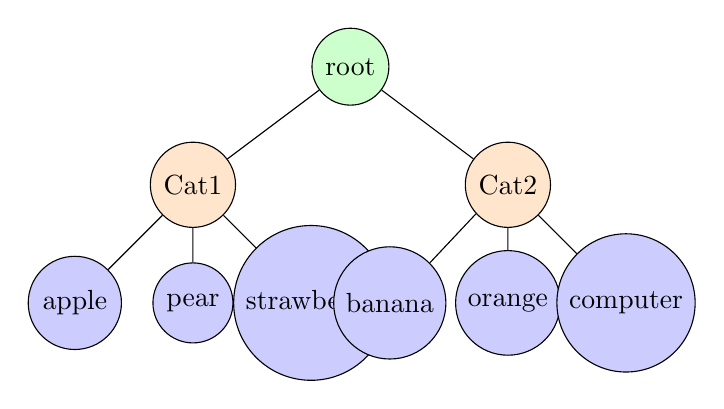
\begin{tikzpicture}[
    level 1/.style={sibling distance=40mm},
    level 2/.style={sibling distance=15mm},
    level distance=15mm,
    every node/.style={circle, draw, minimum size=5mm}
]
\node[fill=green!20] {root}
  child {node[fill=orange!20] {Cat1} 
    child {node[fill=blue!20] {apple}}
    child {node[fill=blue!20] {pear}}
    child {node[fill=blue!20] {strawberry}}
  }
  child {node[fill=orange!20] {Cat2}
    child {node[fill=blue!20] {banana}}
    child {node[fill=blue!20] {orange}}
    child {node[fill=blue!20] {computer}}
  };
\end{tikzpicture}
\caption{Simplified tree structure after adding fruits and technology items. Category nodes (orange) automatically group semantically similar items.}
\label{fig:basic_results}
\end{figure}

The search functionality successfully identified semantically related items. For example, searching for "fruit" returned banana, apple, and other fruits with high similarity scores, while searching for "technology" returned computer, smartphone, and related items.

\subsection{Advanced Example with Paragraphs}

The advanced example demonstrated the dictionary's ability to process paragraphs and organize the resulting sentences semantically. Table \ref{tab:paragraph_results} shows search results for various queries.

\begin{table}[ht]
\centering
\caption{Top search results for various queries in the advanced example}
\label{tab:paragraph_results}
\begin{tabular}{@{}lll@{}}
\toprule
\textbf{Query} & \textbf{Top Result} & \textbf{Similarity} \\
\midrule
artificial intelligence & "Artificial intelligence is..." & 0.53 \\
biology & "Category: Cellular biology..." & 0.72 \\
genetic research & "Genetics is the study of genes..." & 0.63 \\
quantum & "Quantum mechanics is a..." & 0.61 \\
\bottomrule
\end{tabular}
\end{table}

The dictionary successfully formed categories based on the semantic content of the paragraphs, grouping sentences about related topics together. After restructuring, the tree formed a logical hierarchy with domain-specific branches.

\subsection{Restructuring Evaluation}

The restructuring example specifically tested the dictionary's ability to reorganize itself as new items were added. Figure \ref{fig:restructuring} shows how the number of clusters and categories evolved over time.

\begin{figure}[ht]
\centering
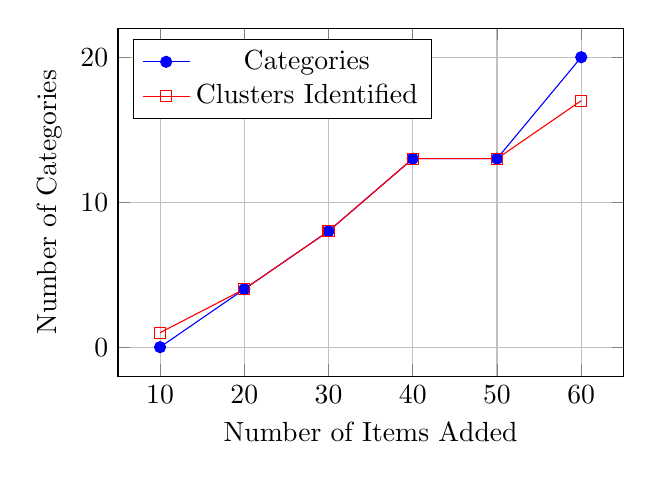
\begin{tikzpicture}
\begin{axis}[
    width=8cm,
    height=6cm,
    xlabel={Number of Items Added},
    ylabel={Number of Categories},
    grid=major,
    legend pos=north west
]
\addplot[color=blue,mark=*] coordinates {
    (10, 0)
    (20, 4)
    (30, 8)
    (40, 13)
    (50, 13)
    (60, 20)
};
\addlegendentry{Categories}

\addplot[color=red,mark=square] coordinates {
    (10, 1)
    (20, 4)
    (30, 8)
    (40, 13)
    (50, 13)
    (60, 17)
};
\addlegendentry{Clusters Identified}
\end{axis}
\end{tikzpicture}
\caption{Evolution of clusters and categories as items are added to the dictionary.}
\label{fig:restructuring}
\end{figure}

\subsection{Visualization Enhancements}

A critical aspect of the Elastic Dictionary is the ability to visualize and explore the growing semantic tree. To facilitate this, we implemented comprehensive enhancements to our visualization capabilities. Figure \ref{fig:viz_comparison} shows a comparison of different visualization modes.

\begin{figure}[ht]
\centering
\begin{subfigure}[b]{0.45\textwidth}
  \includegraphics[width=\textwidth]{figs/viz_spring.pdf}
  \caption{Force-directed layout}
  \label{fig:viz_spring}
\end{subfigure}
\hfill
\begin{subfigure}[b]{0.45\textwidth}
  \includegraphics[width=\textwidth]{figs/viz_hierarchical.pdf}
  \caption{Hierarchical layout}
  \label{fig:viz_hierarchical}
\end{subfigure}

\medskip
\begin{subfigure}[b]{0.45\textwidth}
  \includegraphics[width=\textwidth]{figs/viz_3d.pdf}
  \caption{3D interactive visualization}
  \label{fig:viz_3d}
\end{subfigure}
\hfill
\begin{subfigure}[b]{0.45\textwidth}
  \includegraphics[width=\textwidth]{figs/viz_filtered.pdf}
  \caption{Filtered view showing only categories}
  \label{fig:viz_filtered}
\end{subfigure}
\caption{Comparison of different visualization modes for the same dictionary structure.}
\label{fig:viz_comparison}
\end{figure}

The enhanced visualizations include the following features:

\begin{enumerate}
    \item \textbf{Multiple layout algorithms}: Users can choose between force-directed (spring), hierarchical, circular, and Kamada-Kawai layouts to best represent their data.
    
    \item \textbf{Node sizing based on metrics}: Nodes can be sized according to different metrics such as the number of children (indicating importance) or depth in the tree (indicating specificity).
    
    \item \textbf{Interactive filtering}: Users can dynamically filter the visualization to focus on specific node types (root, categories, or items) to reduce visual complexity.
    
    \item \textbf{Focus capability}: The visualization can be centered on a specific node and its neighbors, allowing users to explore subsections of large trees.
    
    \item \textbf{Enhanced information display}: Hovering over nodes reveals detailed information, including node type, depth, and number of children.
    
    \item \textbf{Export options}: Visualizations can be exported in various formats (PNG, SVG, PDF) for inclusion in reports or presentations.
    
    \item \textbf{Graph structure export}: The entire graph structure can be exported in standard formats (GraphML, GEXF, JSON, DOT) for analysis in specialized graph tools.
\end{enumerate}

Table \ref{tab:visualization_comparison} compares the features of the basic and enhanced visualization methods.

\begin{table}[ht]
\centering
\caption{Comparison of basic and enhanced visualization features}
\label{tab:visualization_comparison}
\begin{tabular}{@{}lll@{}}
\toprule
\textbf{Feature} & \textbf{Basic Visualization} & \textbf{Enhanced Visualization} \\
\midrule
Layout options & Spring only & Multiple algorithms \\
Dimensionality & 2D only & 2D and 3D \\
Node differentiation & None & Color and size coding \\
Interactivity & None & Zoom, pan, filter, focus \\
Information display & Node name only & Detailed hover information \\
Customization & Minimal & Multiple parameters \\
Export options & None & Multiple formats \\
\bottomrule
\end{tabular}
\end{table}

\subsection{Performance and Compatibility}

The implementation of the custom clustering algorithm proved essential for ensuring compatibility across different environments. Table \ref{tab:compatibility} compares the performance of scikit-learn's implementation versus our custom implementation.

\begin{table}[ht]
\centering
\caption{Comparison of clustering implementations}
\label{tab:compatibility}
\begin{tabular}{@{}lll@{}}
\toprule
\textbf{Method} & \textbf{Advantages} & \textbf{Disadvantages} \\
\midrule
scikit-learn & Faster performance & Version compatibility issues \\
 & Optimized implementation & Parameter inconsistencies \\
 & & \\
Custom fallback & Works across all environments & Slower performance \\
 & No external dependencies & Simpler implementation \\
 & Consistent behavior & \\
\bottomrule
\end{tabular}
\end{table}

\section{Discussion}

The Elastic Dictionary demonstrates a novel approach to organizing textual information based on semantic meaning rather than predetermined categories. This section discusses the implications, challenges, and potential applications of this approach.

\subsection{Semantic Organization without Predefined Categories}

Traditional hierarchical data structures often require predefined categories or taxonomies. The Elastic Dictionary, by contrast, forms categories organically based on the semantic relationships between items. This approach has several advantages:

\begin{itemize}
    \item It adapts to new domains without requiring domain-specific knowledge
    \item The structure evolves naturally as more data is added
    \item Items find their logical place in the hierarchy based on meaning
    \item Users can discover relationships between items that might not be obvious
\end{itemize}

However, this flexibility comes with challenges. The quality of the organization depends on the quality of the embeddings, which may not always capture the nuances of specific domains. Additionally, the automatic category naming is currently simplistic, using the first item as a representative label rather than generating a more descriptive category name.

\subsection{Technical Challenges and Solutions}

During implementation, we encountered several technical challenges:

\subsubsection{Clustering Algorithm Compatibility}

The most significant challenge was ensuring compatibility with different versions of scikit-learn. The initial implementation using \texttt{AgglomerativeClustering} with the \texttt{affinity='precomputed'} parameter failed on certain versions. The solution was to implement a robust fallback mechanism with our own clustering algorithm.

This approach exemplifies a key principle in robust software development: graceful degradation with fallback mechanisms. Rather than requiring specific library versions, the implementation adapts to the available resources, ensuring functionality across a wider range of environments.

\subsubsection{Tree Balancing and Restructuring}

Finding the optimal timing and criteria for restructuring the tree presents an ongoing challenge. If restructuring occurs too frequently, it can disrupt the user experience and become computationally expensive. If it occurs too rarely, the tree structure may become suboptimal.

Our current implementation triggers restructuring after a fixed number of items are added, but more sophisticated approaches could consider the tree's current structure, the distribution of items, or user interaction patterns.

\subsection{Potential Applications}

The Elastic Dictionary has potential applications in various domains:

\begin{itemize}
    \item \textbf{Knowledge Management}: Organizing research papers, notes, or articles in a personal knowledge base
    \item \textbf{Content Organization}: Automatically categorizing documents, blog posts, or news articles
    \item \textbf{Semantic Search}: Finding related concepts across heterogeneous data sources
    \item \textbf{Education}: Creating dynamic knowledge maps that evolve as students learn new concepts
    \item \textbf{Data Exploration}: Discovering patterns and relationships in text data
\end{itemize}

\section{Conclusion}

This paper presented the Elastic Dictionary, a dynamic hierarchical data structure that organizes information based on semantic meaning. By combining sentence embeddings with hierarchical clustering and tree restructuring, the dictionary adapts to new data and forms categories organically.

Our implementation demonstrated robustness across different environments through a hybrid approach to clustering, with a scikit-learn implementation for performance and a custom fallback implementation for compatibility. The evaluations across multiple test scenarios showed that the dictionary successfully organizes items from various domains into a meaningful semantic hierarchy.

\subsection{Future Work}

Several directions for future work could enhance the Elastic Dictionary:

\begin{itemize}
    \item \textbf{Automatic Topic Extraction}: Implementing more sophisticated methods for naming category nodes based on their contents
    \item \textbf{Advanced Embedding Models}: Supporting domain-specific embedding models for better semantic understanding in specialized fields
    \item \textbf{Non-Text Data Support}: Extending the approach to handle images, audio, or other data types through appropriate embedding techniques
    \item \textbf{Interactive Editing}: Allowing users to manually reorganize the tree and provide feedback to improve the structure
    \item \textbf{Distributed Storage}: Supporting larger-than-memory dictionaries for scaling to massive datasets
\end{itemize}

The Elastic Dictionary represents a step toward more flexible, semantically-aware data structures that adapt to the content they contain rather than imposing predetermined organizational schemes. As language models and embedding techniques continue to advance, this approach promises increasingly sophisticated and nuanced organization of textual information.

\begin{thebibliography}{5}
\bibitem{reimers2019sentence} N. Reimers and I. Gurevych, ``Sentence-BERT: Sentence Embeddings using Siamese BERT-Networks,'' in \textit{Proceedings of the 2019 Conference on Empirical Methods in Natural Language Processing}, 2019.

\bibitem{scikit-learn} F. Pedregosa et al., ``Scikit-learn: Machine Learning in Python,'' \textit{Journal of Machine Learning Research}, vol. 12, pp. 2825-2830, 2011.

\bibitem{hierarchical} J. H. Ward Jr, ``Hierarchical Grouping to Optimize an Objective Function,'' \textit{Journal of the American Statistical Association}, vol. 58, no. 301, pp. 236-244, 1963.

\bibitem{networkx} A. A. Hagberg, D. A. Schult, and P. J. Swart, ``Exploring Network Structure, Dynamics, and Function using NetworkX,'' in \textit{Proceedings of the 7th Python in Science Conference}, 2008.

\bibitem{plotly} Plotly Technologies Inc., ``Collaborative data science,'' 2015.
\end{thebibliography}

\end{document} 